% !Mode:: "TeX:UTF-8"

\chapter[面向短期交通数据缺失场景的填充算法]{面向短期交通数据缺失场景的填充算法}[]
%15页
\section{引言}
在上一章节中,我们主要针对交通缺失值对其时间分布特性的影响问题进行了相关探究。通过借鉴grui模型,在biconvgru模型的基础上进行扩展操作,设计了一个新型的模型biconvgrui。本章主要研究的问题是探究交通缺失值对其空间分布特性的影响问题。尽管多流变分自编码器MTSVAE能够很好地处理交通缺失值对时间分布特性的影响问题,但是它也没有考虑交通缺失值对其空间分布特性的影响问题。同时,多流变分自编码器在处理交通数据时,没有考虑不同时间窗长度的交通数据间的相互影响。即是默认它们之间是相互独立的,这样的假设会导致模型不能提取准确的时间特征。本章中将交通数据按照邻近(Closeness)栅格数据,周期(Period)栅格数据和趋势(Trend)栅格数据三种时间长度进行划分数据集。为了解决以上问题,本章节的模型采用三层biconvgrui模型处理三种不同时间窗长度的交通数据。一个层次的biconvgrui模型处理一种时间窗长度的交通数据。当前层次的biconvgrui模型处理完当前的交通数据之后,就将得到的隐变量结果传递到下一层biconvgrui模型中,跟待处理的交通数据进行拼接,再送到对应的biconvgrui模型中进行处理。同时,为使得新设计的模型具备提取含有缺失值的交通数据的空间分布,本章使用了轻量级的可学习的双向注意力机制来动态地更新掩膜张量,它能够使得模型在补全阶段使网络更加注重于确实位置的填充。最后,为使得模型具备更好的生成能力,本章使用带有标准化流的变分自编码器处理交通数据的缺失值填充问题。最后,本章节优化了模型的目标函数,使其不仅能高效地填充输入数据地缺失值,还能保证高层空间特征模型地准确性。

%\ref{sec4_4}节介绍轻量级可学习双向注意力图,它在缺失值填充算法中占有重要的作用
%本章的行文安排如下:\ref{sec4_2}节对问题进行了简短地描述;\ref{sec4_3}节介绍了所提出的基于掩膜注意力的变分自编码器填充模型,包括模型整体架构和不同部分的阐述;\ref{sec4_5}节介绍了基于变分自编码器的改进的目标函数;\ref{sec4_6}节提出了模型的训练算法;\ref{sec4_7}节为本章实验及结果分析;\ref{sec4_8}节为本章小结。

\section{问题描述} \label{sec4_2}
本章节在上一章节需要处理的问题的基础上,需要设计一个针对于带有缺失值的数据的卷积模型。同时,将交通栅格数据中的缺失值进行填充,使得生成数据和真实值尽可能相近。
\section{模型架构} \label{sec4_3}
为探究不同时间窗长度的交通数据间的时间相关性,以及提取带有缺失值的空间分布特性。本章节提出了一个多层Attention-Biconvgrui时空变分自编码器(\textit{MCST-VAE}),它的整体架构图如图\ref{framework}所示,这个框架主要包括了以下三个关键的设计思路:1)使用可学习的双向注意力的卷积模块来动态地更新掩膜张量,它能够使得模型在补全阶段使网络更加注重于确实位置的填充;2)使用多层Attention-Biconvgrui模型处理不同时间窗长度的模型,并探究不同时间窗长度数据的时间相关性;3)使用标准化流技术,将一个简单的对角高斯分布通过一系列可迭代的链式函数映射,转换成一个更加复杂的分布。

\begin{figure}[htbp]
\centering
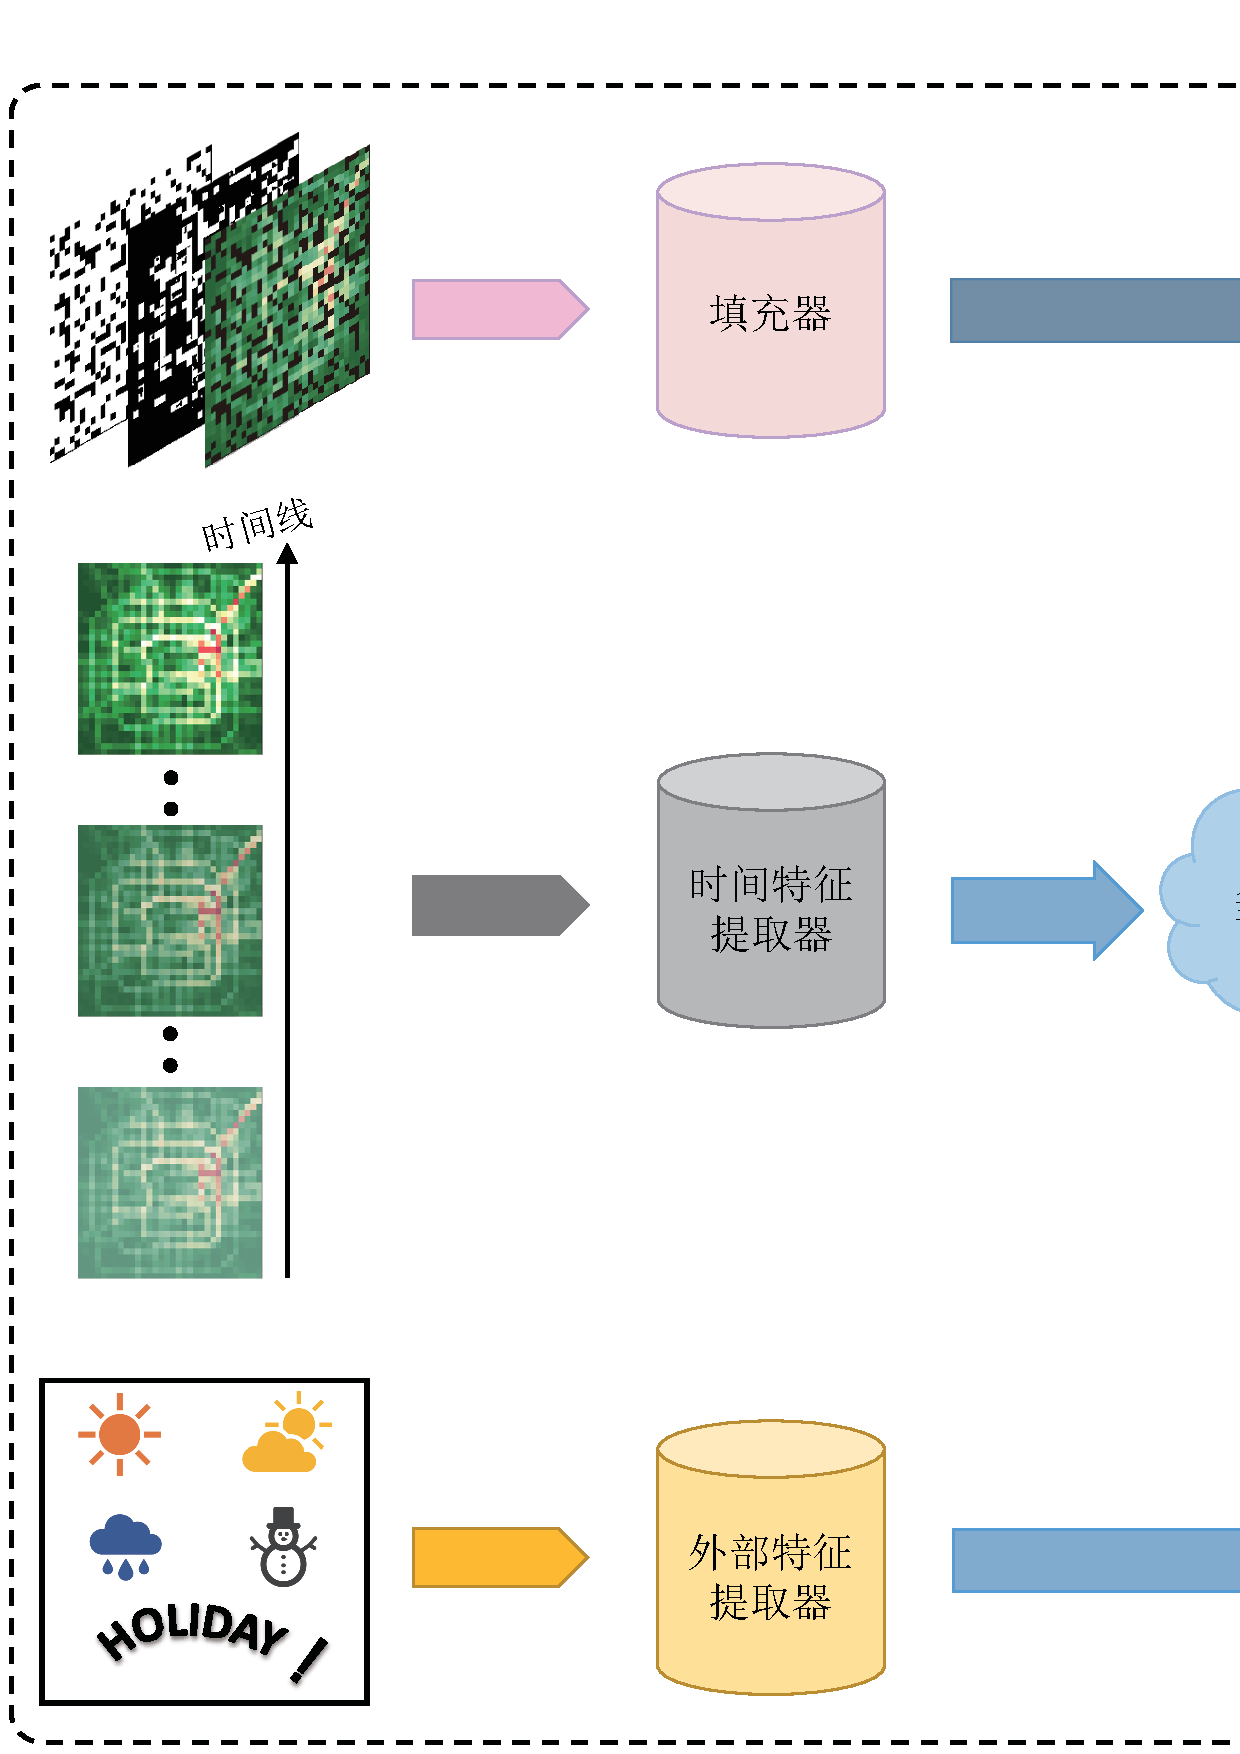
\includegraphics[width = \textwidth]{framework.pdf}
\caption{\textit{ST-LBAVAE}的整体架构图 \label{framework}}
\end{figure}

多层Attention-Biconvgrui时空变分自编码器(\textit{MCST-VAE})由以下三个部分构成。首先是基于可学习的双向注意力图的卷积模块,多层Attention-Biconvgrui模块以及基于标准化流的变分自编码器。以下将按照以上的顺序依次介绍这三部分内容。

\subsection{基于可学习的双向注意力图的卷积模块}
考虑到短期交通数据的缺失值填充场景可以使用历史时刻的完整数据作为参考,因此可以通过对历史数据进行分析来初步提供可能的时间模式,且对时间特征器的设计不需要如填充器一样考虑缺失值的处理问题。

普通卷积模块在处理不含缺失值的数据时取得了良好的效果,但是,交通数据的缺失值带有随机性,即是在雷达图上的缺失地点是不确定的,在时间戳上的缺失时间点也是不确定的,而且不同雷达图上的数值缺失也是不确定的。因而本文需要探求一些新的方法来对这种带有缺失值的交通数据进行有效的建模。针对于在时间戳上的缺失时间点的不确定问题,本文的第一章内容已经设计了$Biconvgrui$模块对带有缺失值的交通数据的时间分布进行有效的建模。为了有效解决普通卷积对雷达图上的数值缺失不敏感问题,本文利用基于可学习的双向注意力图的卷积模块解决此问题。这个方法被左旺孟团队在2019年提出,该方法主要使用了端到端的模型实现了特征再标准化和掩膜矩阵动态更新的效果。具体的表现方式为当特征图在不断地向前传播时,对应的掩膜矩阵$M$也需要不断地更新。即是当特征图在不断地进行采样操作时,对应的观测值也需要进行同步的更新,这种更新的方式主要就是对于掩膜矩阵$M$的持续化更新。参照原论文的方式,具体的更新公式如下所示:

\vspace{-1em}
\begin{subequations}
\begin{align}
\mathbf{F}_{t}^{conv} & = \mathbf{W}^{T}_{pw}f_{bn}(\mathbf{W}^{T}_{dw}\mathbf{F}^{in}_t) \label{dsc_eq} \\
\mathbf{M}^{c}_{t} & = \mathbf{W}^{T}_{m}\mathbf{M}_t  \label{mc_eq}\\
\mathbf{F}_{t}^{out} & = \mathbf{F}_{t}^{conv} \odot f_{A}(\mathbf{M}^{c}_{t})  \label{fr_eq}\\
\mathbf{M}^{'}_{t} & = f_{M}(\mathbf{M}^{c}_{t}) \label{mu_eq},
\end{align}
\end{subequations}

在式子中,$F_in$为模块的输入,$F_conv$为操作的输出,$W_dw$和$W_pw$为卷积操作的参数,在式子中,$W_m$为掩膜卷积操作的参数。在式子中,$\odot$表示哈达玛乘积(Element-wise Product),$f_{A}(\mathbf{M}^{c}_{t})$为可学习的注意力图,具体式子如下所示:
\begin{equation}
    f_{A}(\mathbf{M}^{c}_{t})=
   \begin{cases}
   	\alpha \exp{\big (-\beta(\mathbf{M}^{c}_{t} - \mu)^2 \big)} &\mbox{,若 $\mathbf{M}^{c}_{t} < \mu$}\\
   	1 + (\alpha - 1) \exp{\big ( - \gamma(\mathbf{M}^{c}_{t} - \mu)^2 \big)} &\mbox{,其它}
   \end{cases}
\end{equation}
其中$\alpha$,$\beta$,$\mu$,$\gamma$均为可学习的参数,初始值设置与文献\cite[8861]{xie2019image}同。式子\eqref{mu_eq}表示掩膜的动态更新,具体的更新函数如下所示:
\begin{equation}
    f_{M}(\mathbf{M}^{c}_{t}) = \left [ ReLU(\mathbf{M}^{c}_{t}) \right ]^{\theta}.
\end{equation}

与前向注意力图不同的是,反向注意力图的作用在于聚焦缺失值的修复,即如何运用编码器得到的隐变量信息进行缺失值的预测,所以本文使用与掩膜矩阵$M_t$相反的输入$1-M_t$作为反向注意力图模块的输入。

\begin{figure}[htbp] 
	\centering 
	\subfigure[邻近性]{
		\begin{minipage}[htbp]{0.31\textwidth}
			\includegraphics[width=1\textwidth]{closeness} \label{closeness}
		\vspace{-1em}
		\end{minipage}	
	}
	\subfigure[周期性]{
		\begin{minipage}[htbp]{0.31\textwidth}
			\includegraphics[width=1\textwidth]{period} \label{period}
		\vspace{-1em}
		\end{minipage}
	}
	\subfigure[趋势性]{
		\begin{minipage}[htbp]{0.31\textwidth}
			\includegraphics[width=1\textwidth]{trend} \label{trend}
		\vspace{-1em}
		\end{minipage}
	}
	\caption{居民区域入流量(Inflow)的时间依赖性\cite[4]{zhang2017deep}} \label{residual}
\end{figure}

\subsection{多层Attention-Biconvgrui模块}
多层$Biconvgrui$模块是(\textit{MCSTVAE})的一个子模型,它增强了模型提取不完整数据的时间分布特性的能力,并且使得模型能够提取不同时间窗长度的时间相关性。在本章节中,为了进一步增强$Biconvgrui$模块对于交通数据的缺失值的捕捉能力,使用基于可学习的双向注意力图的卷积模块来替换普通的卷积模块。同时,将交通数据按照邻近性,周期性和趋势性三种时间长度划分成三个不同的数据集。同时,将处理邻近性数据集的$Biconvgrui$模型定义为$B_c$, 处理周期性数据集的$Biconvgrui$模型定义为$B_p$,以及处理趋势性数据集的$Biconvgrui$模型定义为$B_t$。给定数据$X_c$,$X_p$以及$X_t$和相应的掩膜矩阵$M_c$,$M_p$和$M_t$作为多层$Biconvgrui$模块的输入,整个多层$Biconvgrui$模块的计算过程,可以用以下公式表示:

\vspace{-1em}
\begin{subequations}
\begin{align}
\mathbf{h}_{c} & = \mathbf{B}_{c}([\mathbf{X}_{c},\mathbf{h}_0]) \label{dsc_eq} \\
\mathbf{F}^{c}_{conv} & = \mathbf{W}^{c}_{pw}\mathbf{M}_t  \label{mc_eq}\\
\mathbf{F}_{t}^{out} & = \mathbf{F}_{t}^{conv} \odot f_{A}(\mathbf{M}^{c}_{t})  \label{fr_eq}\\
\mathbf{M}^{'}_{t} & = f_{M}(\mathbf{M}^{c}_{t}) \label{mu_eq},
\end{align}
\end{subequations}

交通流量可以被多种复杂的外部因素所影响,例如气象、节假日等,如图\ref{extra_features}所示。图\ref{storm}显示了极端天气对于城市人流量的影响,其中红色曲线表示2013年8月11日北京某办公区域的交通入流量,绿色曲线表示2013年8月18日同区域的入流量情况。从图中可以看出当11日下午发生强降雨天气时,该办公区域的人员在下班时间段相较于平时,其入流量出现了骤减的趋势,而18日下午的天气情况为晴朗。图\ref{holiday}展示了2016年北京市某办公区域春节期间(红色)与春节假期结束后一周(绿色)的人流量之间的差异,可以看出在春节期间办公区域的交通入流量比非节假日期间要少很多。因此,将这些额外因素作为极端事件下缺失值的填充是有必要的,它能在特殊情况下为模型提供一些辅助的信息。本文考虑了气象情况、节假日和周末这些外部因素,其中气象情况又包含了天气、气温和风速信息。

\begin{figure}[htbp] 
	\centering 
	\subfigure[强降雨和正常天气下的城市人流量]{
		\begin{minipage}[htbp]{0.48\textwidth}
			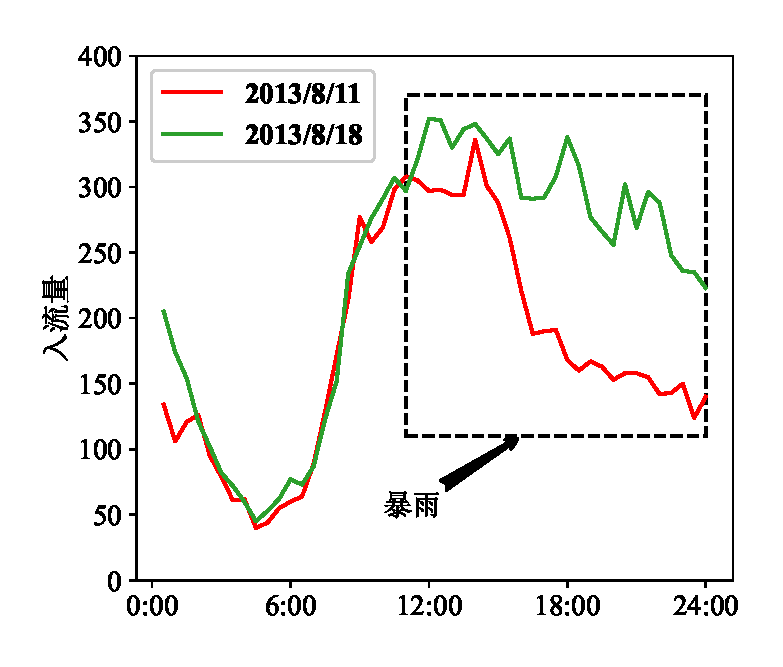
\includegraphics[width=1\textwidth]{storm2} \label{storm}
%		\vspace{-1em}
		\end{minipage}	
	}
	\subfigure[(非)节假日的城市人流量]{
		\begin{minipage}[htbp]{0.48\textwidth}
			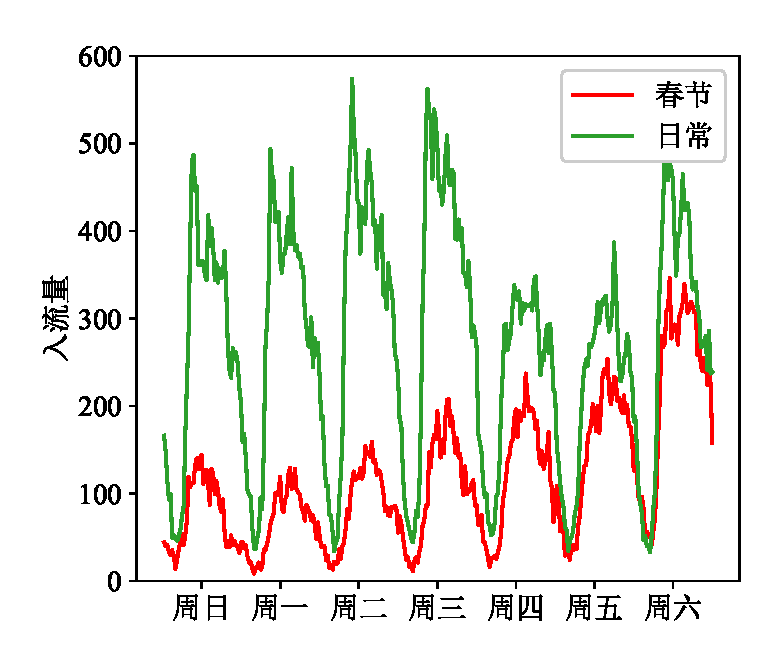
\includegraphics[width=1\textwidth]{holiday2} \label{holiday}
%		\vspace{-1em}
		\end{minipage}
	}
	\caption{外部因素对北京市某办公区域入流量的影响} \label{extra_features}
\end{figure}

考虑到额外数据的离散性,本文将离散数据用独热编码(One-Hot Encoding)的方式进行处理,这样单个离散的值便可以用向量的形式来表示,向量的长度即为离散值的状态数,进而实现了将离散属性数据映射到欧式空间的目的,便于计算离散属性数据之间的相似性。以工作日/周末特征为例,本文用一个八位只有0和1的二值向量来表示它。前七位表示周一至周日,最后一位表示是否为非工作日,若为非工作日,则标记为1,比如星期一用独热编码后的向量为$(1, 0, 0, 0,0,0,0,1)$。

本文设计了外部特征提取器来完成外部信息的表示,具体结构如图\ref{extra_extractor}所示。假设处理后的额外数据为$\mathbf{E}_t$,首先使用一个嵌入层加$ReLU$激活函数将其从高维空间非线性地映射到低维空间,用于特征的压缩,同时也可以减少网络训练的参数量,接着最后使用另一个全连接层和$Reshape$操作来保证最后输出的形状能与待填充栅格图$\mathbf{X}_t$相匹配,便于之后的多特征融合,记外部特征提取器的输出为$\mathbf{X}_t^{ext}$。

\begin{figure}[htbp]
\centering
\includegraphics[width = 0.9\textwidth]{extra_extractor.pdf}
\vspace{-4em}
\caption{外部特征提取器的结构图 \label{extra_extractor}}
\end{figure}

\subsection{填充器}
本文设计了带有轻量级的双向可学习注意力图的变分自编码器来进行缺失值的填充,如图\ref{filler}所示。它包含编码器、随机隐变量表达层和解码器,编码器由多个下采样层组成,解码器由多个上采样层组成。

\begin{figure}[htbp]
\centering
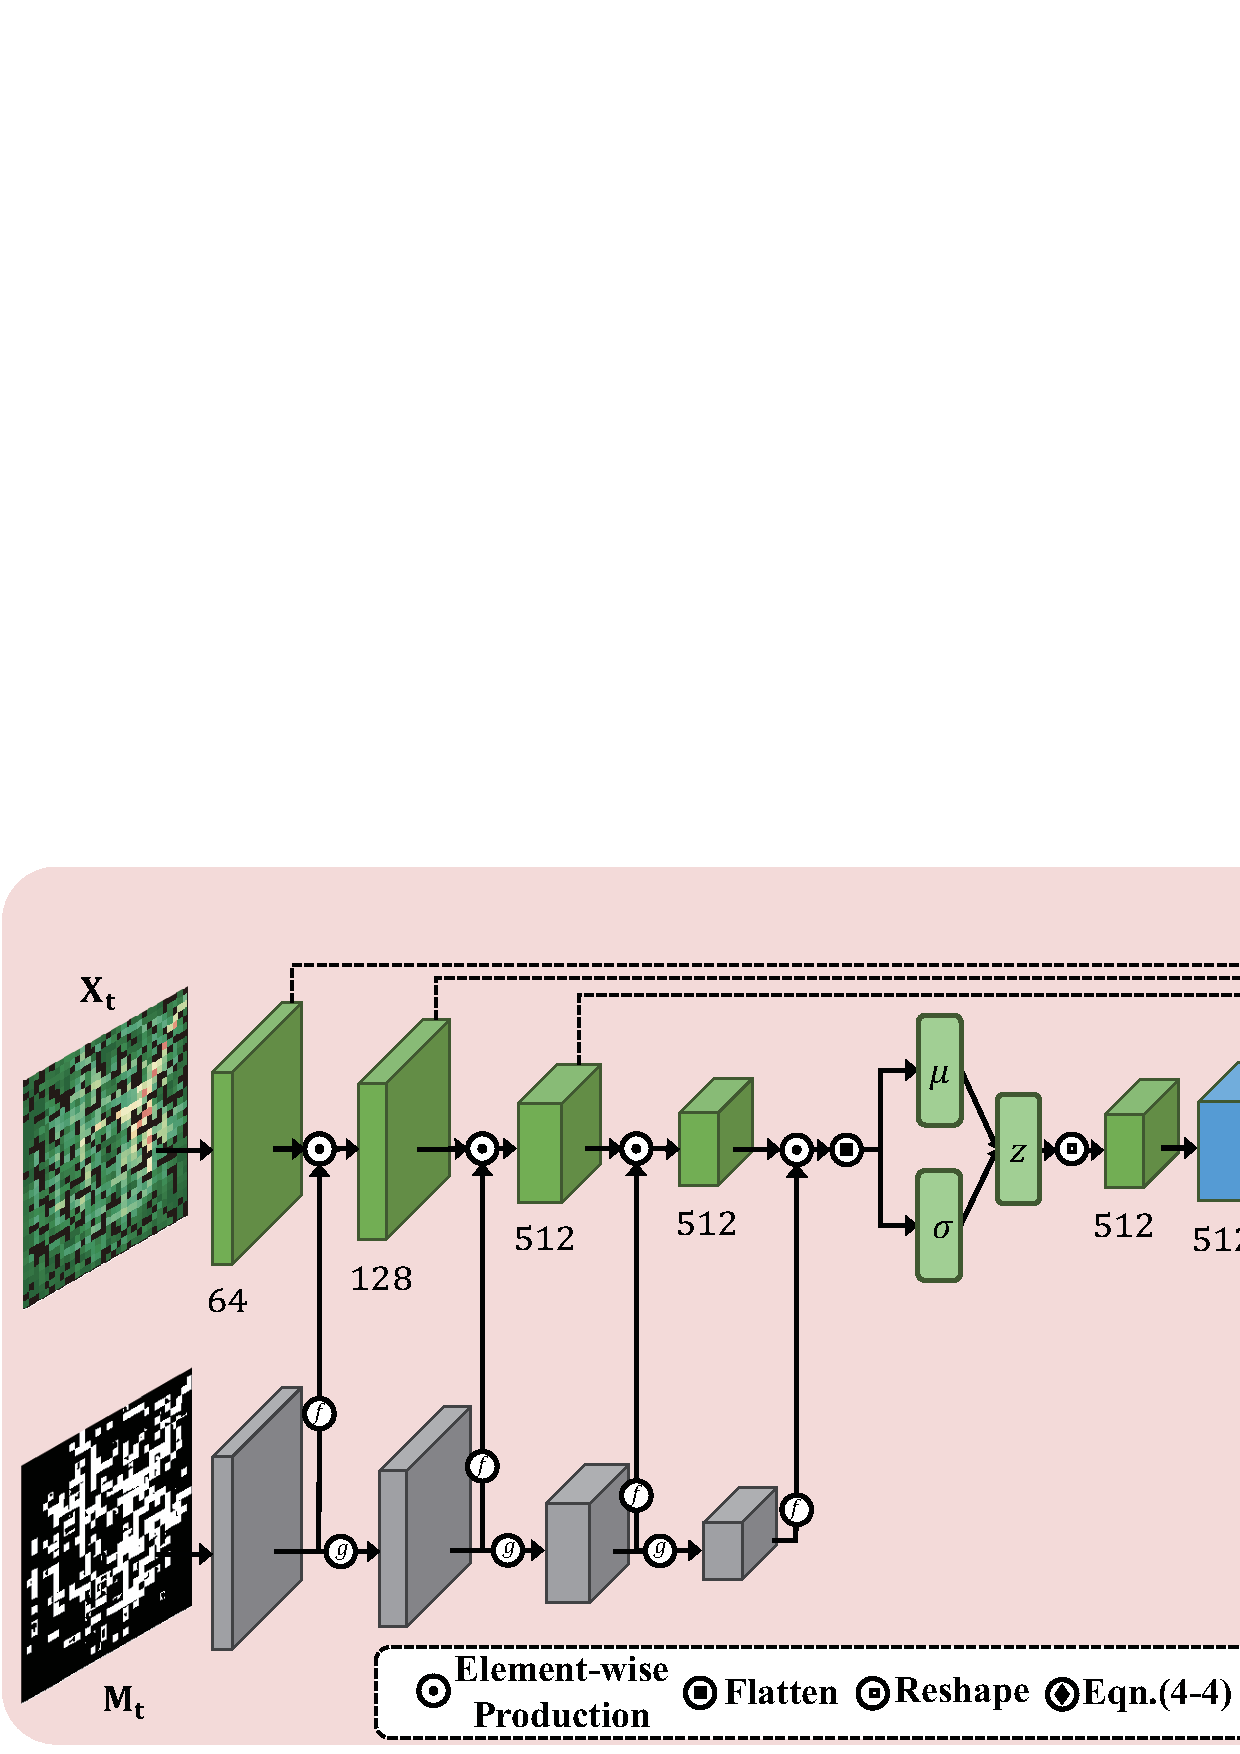
\includegraphics[width = \textwidth]{filler.pdf}
\vspace{-1em}
\caption{轻量级双向可学习注意力变分自编码器 \label{filler}}
\end{figure}

填充器以待填充的交通栅格图$\mathbf{X}_t$作为输入,同时还使用了待填充数据的掩膜矩阵$\mathbf{M}_t$,在$\mathbf{M}_t$中,元素值1表示栅格图$\mathbf{X}_t$中对应位置的值可以被观测到,0表示对应位置的值是缺失值。$\mathbf{X}_t$和$\mathbf{M}_t$每次经过下采样层,其特征图的尺寸都会缩减为原来的一半,但是通道数会翻倍;相反,经过上采样层的时候,特征图的尺寸会扩大为原来的两倍,但是通道数会减少为原来的一半。由多个下采样层组成的编码器输出随机隐变量的均值$\mu$和标准差$\sigma$,再通过重参数化技巧得到随机隐变量$z$,主要过程与式子\eqref{vae_equation_d}一致。接着随机隐变量$z$通过解码器上采样后得到初步还原的栅格图$\mathbf{X}_{t}^{'}$,在解码阶段还用到了与$\mathbf{M}_t$相反的输入$1-\mathbf{M}_t$11。

\begin{figure}[htbp] 
	\centering 
	\subfigure[前向可学习注意力图]{
		\begin{minipage}[htbp]{0.48\textwidth}
			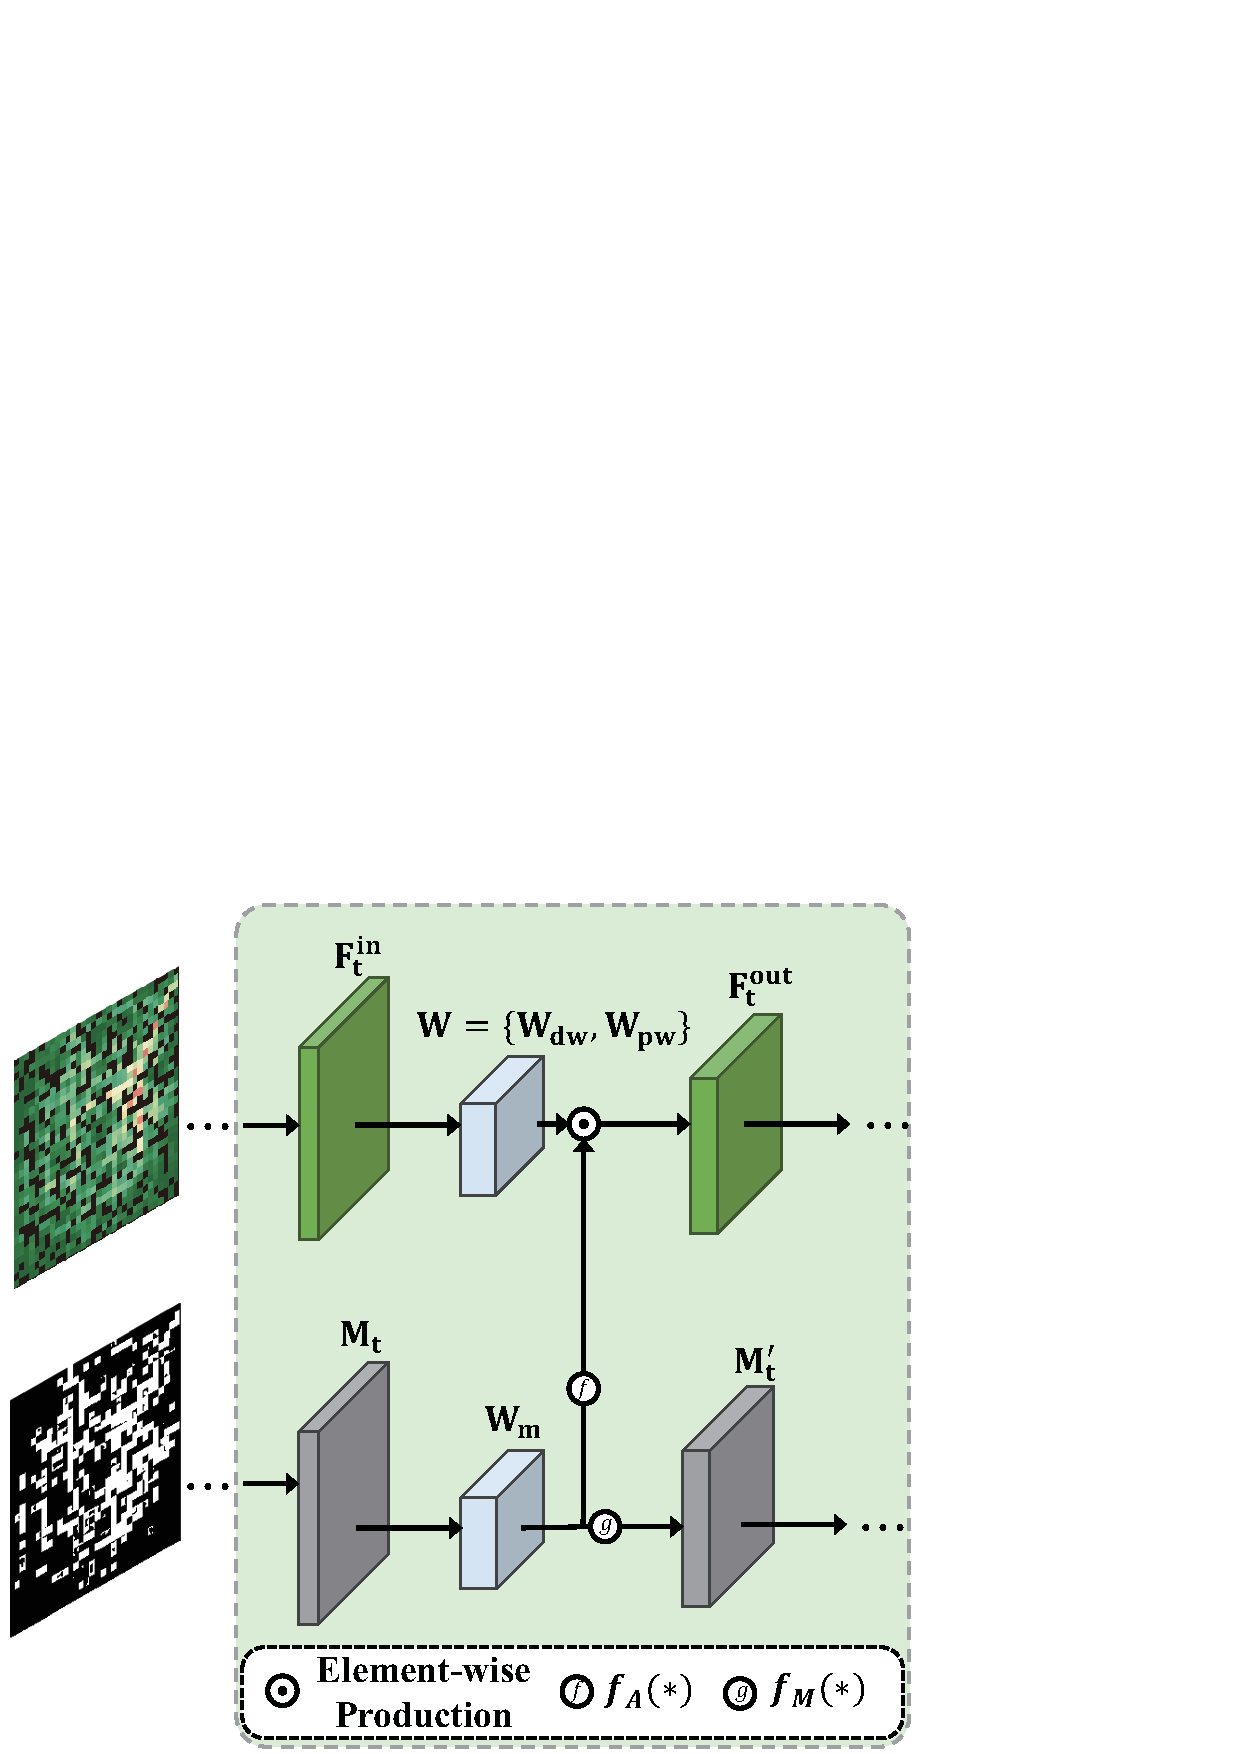
\includegraphics[width=1.03\textwidth]{forward_llbam.pdf} \label{forward_llbam}
%		\vspace{-1em}
		\end{minipage}	
	}
	\subfigure[反向可学习注意力图]{
		\begin{minipage}[htbp]{0.48\textwidth}
			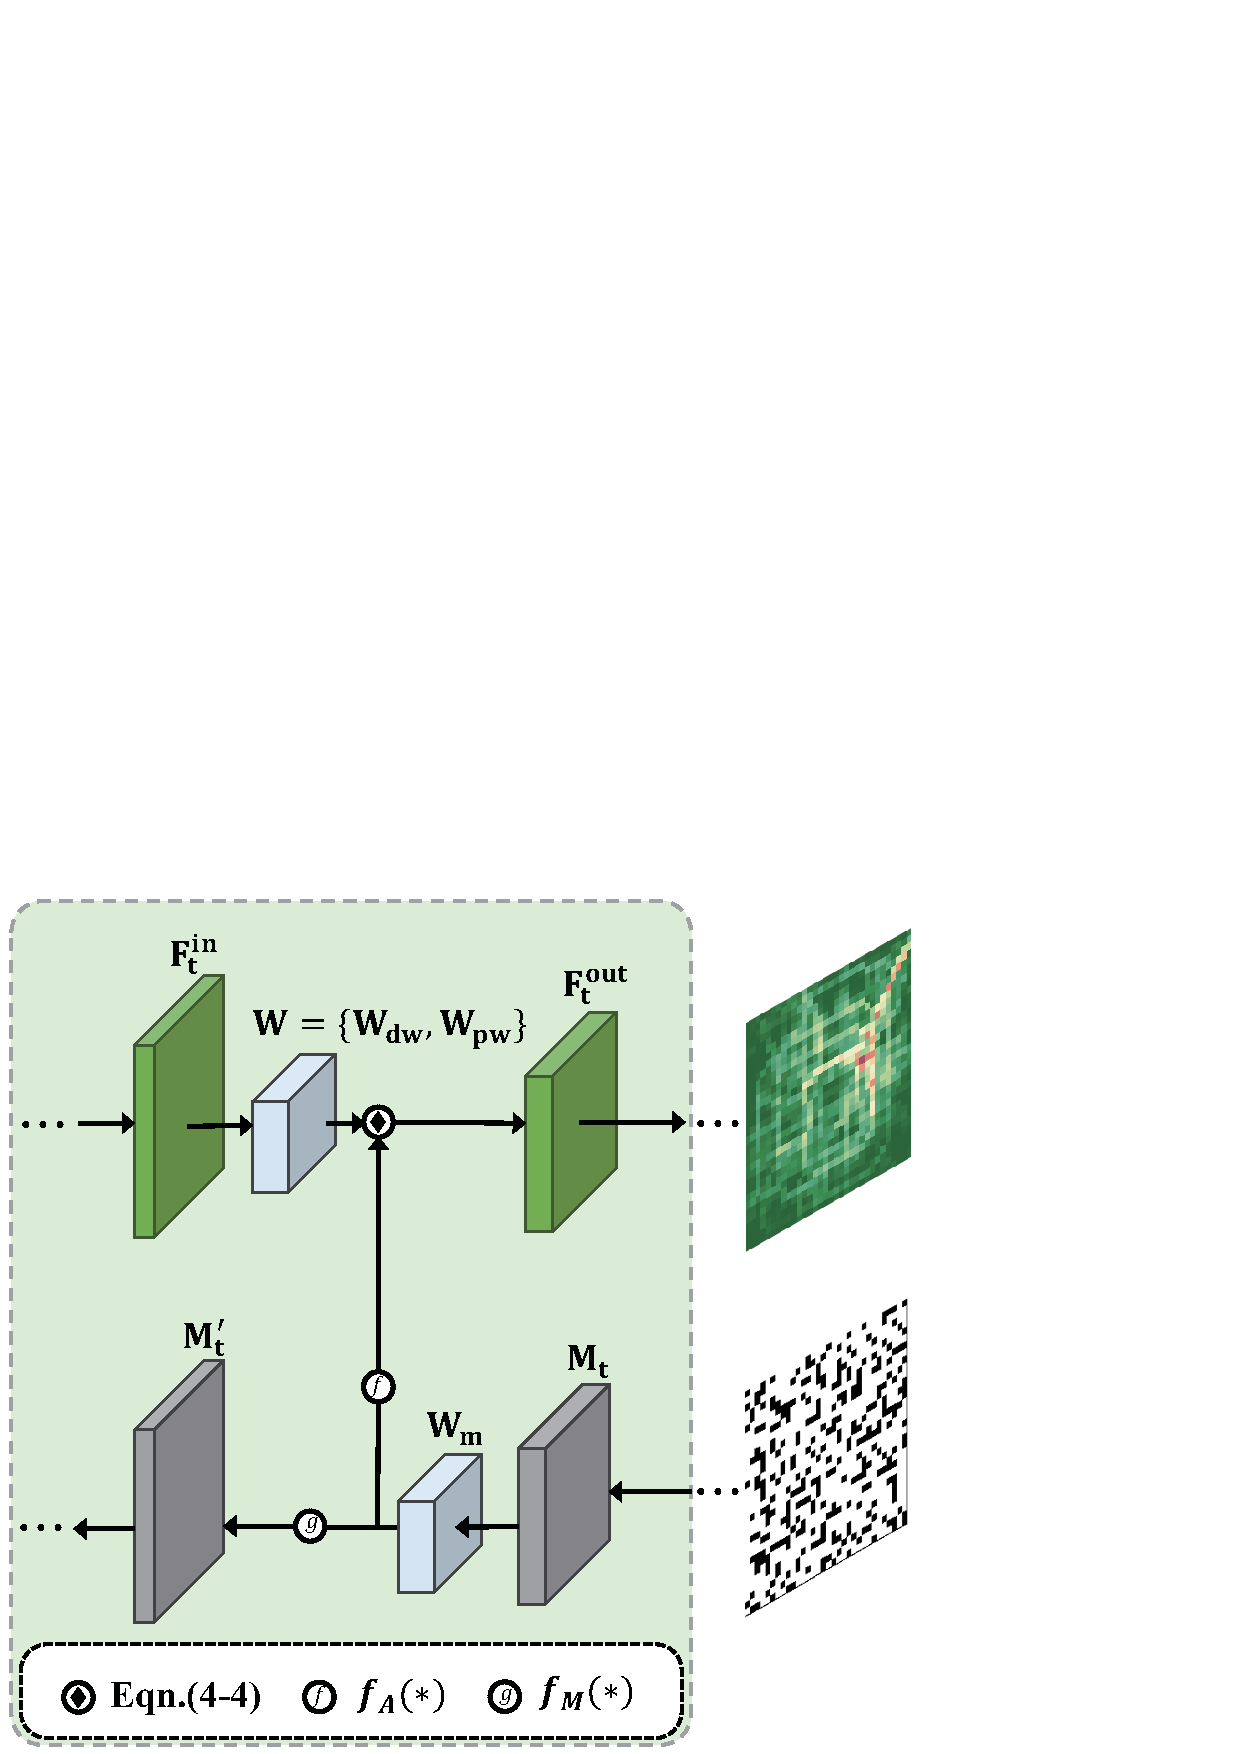
\includegraphics[width=1.0\textwidth]{reverse_llbam.pdf} \label{reverse_llbam}
%		\vspace{-1em}
		\end{minipage}
	}
	\caption{轻量级双向可学习注意力图模块} \label{llbam}
\end{figure}

额外地,考虑到城市交通数据的缺失情况具有随机性,即缺失的地点是不确定的,缺失的时间戳是不确定的,同时缺失的比例也是预先未知的,而当前的基于深度学习的交通数据缺失值填充算法\cite{yu20193d,boquet2019missing}很难处理这种情况。为了模拟实际场景中不规则的交通流的缺失值分布情况,本文利用可学习的双向注意力图模块\cite{xie2019image}解决了此问题,该模块于2019年被左旺孟团队提出,主要以一种端到端的方式来达到特征再标准化和掩膜矩阵动态更新的效果,具体表现为在特征图向前传播的同时,掩膜矩阵也会随之进行动态更新,即随着特征图不断地下采样,对应的观测值的信息也需要不断被更新,而这个更新的指示器就是可更新的掩膜矩阵$\mathbf{M}_t$,本文将其做了模块轻量化的改进,故称为轻量级可学习注意力图,如图\ref{llbam}所示。它主要可以分为四个操作:(1)深度可分离卷积(Depth-wise Separable Convolution);(2)掩膜卷积(Mask Convolution);(3)特征再标准化(Feature Re-Normalization);(4)掩膜更新(Mask Updating)。可用如下式子表示:
\vspace{-1em}
\begin{subequations}
\begin{align}
\mathbf{F}_{t}^{conv} & = \mathbf{W}^{T}_{pw}f_{bn}(\mathbf{W}^{T}_{dw}\mathbf{F}^{in}_t) \label{dsc_eq} \\
\mathbf{M}^{c}_{t} & = \mathbf{W}^{T}_{m}\mathbf{M}_t  \label{mc_eq}\\
\mathbf{F}_{t}^{out} & = \mathbf{F}_{t}^{conv} \odot f_{A}(\mathbf{M}^{c}_{t})  \label{fr_eq}\\
\mathbf{M}^{'}_{t} & = f_{M}(\mathbf{M}^{c}_{t}) \label{mu_eq},
\end{align}
\end{subequations}
在式子\eqref{dsc_eq}中,$\mathbf{F}^{in}_t$为模块的输入,$\mathbf{F}^{conv}_t$为操作(1)的输出,$\mathbf{W}_{dw}$和$\mathbf{W}_{pw}$为深度可分离卷积\cite{chollet2017xception}的两次卷积操作(Depth-wise $\&$ Point-wise Convolution)的参数,两次卷积中穿插了一个批标准化操作$f_{bn}$。相较于普通卷积,深度可分离卷积极大地减少了网络的训练参数,以本文的数据集TaxiBJ中的输入样本为例,输入形状为$[1,32,32]$,则输出形状为$[64,16,16]$的特征图需要使用64个$3 \times 3$的卷积核(参数量为576),而使用深度可分离卷积需要使用1个$3 \times 3$的卷积核和64个$1 \times 1$的卷积核(参数量为73),比较之下后者的训练参数减少了$87\%$。在式子\eqref{mc_eq}中,$\mathbf{W}_m$为掩膜卷积操作的参数。在式子\eqref{fr_eq}中,$\odot$表示哈达玛乘积(Element-wise Product),$f_{A}(\mathbf{M}^{c}_{t})$为可学习的注意力图,具体式子如下所示:
\begin{equation}
    f_{A}(\mathbf{M}^{c}_{t})=
   \begin{cases}
   	\alpha \exp{\big (-\beta(\mathbf{M}^{c}_{t} - \mu)^2 \big)} &\mbox{,若 $\mathbf{M}^{c}_{t} < \mu$}\\
   	1 + (\alpha - 1) \exp{\big ( - \gamma(\mathbf{M}^{c}_{t} - \mu)^2 \big)} &\mbox{,其它}
   \end{cases}
\end{equation}
其中$\alpha$,$\beta$,$\mu$,$\gamma$均为可学习的参数,初始值设置与文献\cite[8861]{xie2019image}同。式子\eqref{mu_eq}表示掩膜的动态更新,具体的更新函数如下所示:
\begin{equation}
    f_{M}(\mathbf{M}^{c}_{t}) = \left [ ReLU(\mathbf{M}^{c}_{t}) \right ]^{\theta}.
\end{equation}

轻量级的可学习注意力图被应用于填充器的编码阶段,用于表示随着特征图不断地下采样,对应的观测值的信息也需要不断被更新,又称为前向注意力图。不难理解,该注意力图主要用于有针对性地提取有效位置的数据的特征。

同时,本文使用U-Net\cite{ronneberger2015u}结构将编码器中第$l$层的特征图与解码器中第$L-l$层的特征图拼接起来作为解码器中第$L-l+1$层的输入。其本质是通过跳跃连接融合不同层次的语义特征,使得特征的表达更加的准确。假设用$\mathbf{F}^{conv}_e$和$\mathbf{F}^{conv}_d$分别表示经过深度可分离卷积后的编码器和解码器的特征图,$\mathbf{M}^{c}_e$和$\mathbf{M}^{c}_d$分别表示编码器和解码器的卷积后的掩膜,基于U-Net结构,则解码器中的特征再标准化操作可以改写为如下式子:
\begin{equation}
	\mathbf{F}_{d}^{out} = \mathbf{F}^{conv}_e \odot f_{M}(\mathbf{M}^{c}_{e}) + \mathbf{F}^{conv}_d \odot f_{M}(\mathbf{M}^{c}_{d}),
\end{equation}
与前向注意力图不同的是,反向注意力图的作用在于聚焦缺失值的修复,即如何运用编码器得到的隐变量信息进行缺失值的预测,故本文使用与掩膜矩阵$M_t$相反的输入$1-M_t$作为反向注意力图模块的输入。

此外,由于输入的只是单时间槽的栅格数据,因此,该填充器使用2D卷积专注于交通流量中空间相关性的建模。



\subsection{多特征融合机制}
关于多特征融合,一般有两种方式,一种是相加操作,另一种是拼接操作。本文首先将填充器输出的特征图$\mathbf{X}_t^{'}$与时间提取器输出的特征图$\widetilde{\mathbf{X}}_t$进行相加,最后将其与外部特征的输出$\mathbf{X}_t^{ext}$进行拼接操作,如下式所示:
\begin{subequations} \label{fusion_eq}
\begin{align}
	H_t(:,c,:,:) & = \mathbf{X}_t^{'}(:,c,:,:) + \widetilde{\mathbf{X}}_t(:,c,:,:), c=0,...,C-1 \\
	H_t(:,C,:,:) & = \mathbf{X}_t^{ext},
\end{align}
\end{subequations}
这样做的原因是时空特征是复杂的,通过相加操作能有助于时空模式的建立,而外部特征会间接地影响时空特征的极端表示,故将其拼接最后通过卷积核大小为$1\times 1$,步长为1的2D卷积操作进行通道特征的融合。



\section{目标函数和模型训练} \label{sec4_5}
为了更好地恢复交通数据的上下文细节和语义特征,本文引入了变分自编码器损失、感知损失和风格损失来训练\textit{ST-LBAVAE}。

(1)\textbf{变分自编码器损失函数}:该损失函数主要由三部分组成,分别为观测值重建误差、缺失值误差和随机隐变量分布的$KL$散度。记真实完整样本为$X$,重建样本为$\hat{X}$,掩膜矩阵为$M$,则观测值重建误差如下式所示:
		\begin{equation}
			Loss_1 = \frac{1}{n}\sum_{i=1}^{n}((X \otimes M)_i - (\hat{X} \otimes M)_i)^2
		\end{equation}
		其中$n$为缺失值的数量,$\otimes$表示元素对位相乘。
		
		缺失值重建误差如下式所示:
		\begin{equation}
			Loss_2 = \frac{1}{n}\sum_{i=1}^{n}((X \otimes (1-M))_i - (\hat{X} \otimes (1-M))_i)^2
		\end{equation}
		
		$KL$散度损失如下式所示:
		\begin{equation}
			Loss_3 = -\frac{1}{2} \sum_{j=1}^{D}\bigg (1+ \log{\sigma_j^2} - \mu_j^2 - \sigma_j^2\bigg )
		\end{equation}
		其中,$D$表示随机隐变量的维数。
		
(2)\textbf{感知损失函数}:变分自编码器损失中的前两项只是简单地计算了真实值与预测值之间的误差,但是忽略了交通数据中更加高层的语义信息。本文通过将真实样本和重建样本分别输入到在Imagenet\cite{russakovsky2015imagenet}上进行了预训练的VGG-16模型\cite{simonyan2014very}来衡量高层特征之间的误差,即感知损失,如下式所示:
		\begin{equation}
			Loss_4 = \frac{1}{N} \sum_{k=1}^{N}\frac{1}{n}\sum_{i=1}^{n}(\mathcal{P}_{k}(X) - \mathcal{P}_{k}(\hat{X}))^2,
		\end{equation}
		其中,$\mathcal{P}_{k}(\cdot)$表示VGG-16模型中第$k$个池化层的特征图。本文使用了其中的三层池化层,即$N=3$。

(3)\textbf{风格损失函数}:为了更好地还原交通数据的上下文信息,本文引入了风格损失函数。它用于衡量由VGG-16模型输出的特征图之间$Gram$矩阵的相似性,假设特征图$\mathcal{P}_{k}(\cdot)$的尺寸为$C_k \times H_k \times W_k$,则风格损失函数如下式子所示:
		\begin{equation}
			Loss_5 = \frac{1}{N} \sum_{k=1}^{N} \frac{1}{n \times C_k^2}\sum_{i=1}^{n}(\mathcal{P}_{k}(X)(\mathcal{P}_{k}(X)^T - \mathcal{P}_{k}(\hat{X})\mathcal{P}_{k}(\hat{X})^T)^2.
		\end{equation}

综合上述五个损失函数,\textit{ST-LBAVAE}的目标函数用如下式子表示:
\begin{equation}
	\mathcal{L} = \lambda_1 Loss_1 + \lambda_2 Loss_2 + \lambda_3 Loss_3 + \lambda_4 Loss_4 + \lambda_5 Loss_5 \label{lbavae_loss}
\end{equation}
其中$\lambda_1=1.0, \lambda_2=6.0, \lambda_3=1.0, \lambda_4=0.05, \lambda_5=120$。
 
本文可以通过梯度下降法优化式子\eqref{lbavae_loss}的方式来线下训练\textit{ST-LBAVAE}。下面给出训练\textit{ST-LBAVAE}模型的伪代码,如下所示。
\begin{algorithm}[htbp]
	\floatname{algorithm}{算法} 
	\renewcommand{\algorithmicrequire}{\textbf{输入:}}
	\renewcommand{\algorithmicensure}{\textbf{输出:}}
	\caption{\quad \textit{ST-LBAVAE} 训练算法}
	\label{alg1}
	\begin{algorithmic}[1]
		\REQUIRE 历史完整数据$\{X_0, X_1, \dots,X_{n-1}  \}$;对应掩膜矩阵$\{M_0, M_1, \dots,M_{n-1}  \}$;外部因素$\{E_0, E_1, \dots,E_{n-1}  \}$;邻近、周期、趋势属性数据片段的长度$l_c, l_p, l_q$;周期定义长度$p$;趋势定义长度$q$。
		
		\ENSURE 学习完参数的\textit{ST-LBAVAE}模型
		
		\textbf{步骤 1}: 构建训练样本集 
		
		\STATE 使用最大最小归一化将数据范围缩到区间$[-1, 1]$
		
		\STATE $\mathcal{D} \longleftarrow \emptyset$
		
		\FOR {$t = 1$ to $n-1$}
			\STATE $\mathcal{S}_c$ = [$X_{t-l_c}, X_{t-({l_c-1})}, \dots, X_{t-1}$]
			\STATE $\mathcal{S}_p$ = [$X_{t-l_p \cdot p}, X_{t-({l_p-1}) \cdot p}, \dots, X_{t-p}$]
			\STATE $\mathcal{S}_q$ = [$X_{t-l_q \cdot q}, X_{t-({l_q-1}) \cdot q}, \dots, X_{t-q}$]
			\STATE 将缺失值用零进行预填充,获得预处理后的样本$\widetilde{X_{t}}$
			\STATE 将元组$(X_t, M_t, \mathcal{S}_c, \mathcal{S}_p, \mathcal{S}_q, \widetilde{X_{t}})$作为一个样本放入数据集$\mathcal{D}$
		\ENDFOR
		
		\textbf{步骤 2}: 训练\textit{ST-LBAVAE}模型
		 
		\STATE 初始化\textit{ST-LBAVAE}中所有可学习的参数
		\REPEAT
		\STATE 随机从$\mathcal{D}$中选择一批次的样本$X_b$
		\STATE $\varphi, \theta \longleftarrow$ 使用Adam优化器更新参数 
		\UNTIL 目标函数$\mathcal{L}$收敛
	\end{algorithmic}  
\end{algorithm}


\section{实验与分析} \label{sec4_7}
本小节首先介绍了实验所需要用的数据集,然后列出了实验环境和模型参数的设置,接着进行了对比实验和模型复杂度的分析,最后给出了消融实验的结果。
\subsection{数据集}
为了定量地评价所提出的模型的填充效果,本文使用了TaxiBJ\cite{zhang2017deep}和BikeNYC\cite{zhang2017deep}数据集,数据集描述如表\ref{tb_dataset}所示。

以上轨迹数据均可通过定义(\ref{def_flow})转换为交通出入流量数据。本文按照五个缺失值比例10\%,30\%,50\%,70\%,90\%随机手动生成相应的数据集。接着使用归一化将数据集数值范围缩放到区间[-1,1]内。对于每个数据集,本文将数据集前90\%的样本作为训练集,剩余的样本作为测试集,又取训练集中的90\%作为验证集。为了防止模型训练产生过拟合现象,我们保存在验证集上损失函数最小的模型参数用于测试。

\subsection{实验设置} \label{setup}
(1)\textbf{实验环境}:本章实验均在GPU服务器上完成,表\ref{env1}给出了实验所采用的软硬件环境的具体细节。

\begin{table}[htbp] \footnotesize
\caption{ 实验软硬件环境} \label{env2}
\vspace{0.5em}\centering\wuhao
\begin{tabular}{cc}
\toprule[1.5pt]
环境 & 参数\\
\midrule[1pt]
操作系统 & Ubuntu 20.04.2.0 LTS \\
内存 & 128GB \\
磁盘 & 1TB SSD \\
处理器 & 英特尔至强Gold 5218R@2.10GHz \\
图形卡 & GeForce RTX 3080 \\
CUDA版本 & 11.1 \\
开发语言 & Python 3.8 \\
深度学习框架 & Pytorch 1.8.1 \\
\bottomrule[1.5pt]
\end{tabular}
\end{table}

(2)\textbf{模型超参设置:}每一个3D卷积模块的卷积核均设置为$3\times 3 \times3$,随机隐变量$z$的长度固定为128,周期定义长度$p$为一天,趋势定义长度$q$为一星期,$l_c$在$\{1, 2, 3, 4\}$中取值,$l_p$在$\{2, 3, 4\}$中取值,$l_q$在$\{2, 3, 4\}$中取值。本实验采用Adam优化器来进行梯度优化,且初始学习率为$10^{-3}$,一阶矩估计和二阶矩估计的指数衰减率分别为$0.5$和$0.9$。最后,模型在TaxiBJ和BikeNYC上的训练周期数均为200。

(3)\textbf{评价指标:}本文采用均方根误差(RMSE)和平均绝对误差(MAE)作为模型评价的指标,具体公式如下所示:
\begin{equation}
\mathrm{RMSE}=\sqrt{\mathbb{E}\big \{ \left\|(1-m) \otimes \left(x-\hat{x}\right)\right\|_{F} \big \}}
\end{equation}
\begin{equation}
\mathrm{MAE}=\mathbb{E}\big \{ \left\|(1-m) \otimes \left(x-\hat{x}\right)\right\|_{1} \big \}
\end{equation}
%\begin{equation}
%\mathrm{NMSE}=\mathbb{E}\bigg \{\frac{\left\|(1-m) \otimes \left(x-\hat{x}\right)\right\|_{F}}{\left\|(1-m) \otimes x\right\|_{F}} \bigg \}
%\end{equation}

\subsection{对比实验结果与分析}
为了验证\textit{ST-LBAVAE}模型在短期交通数据缺失值填充中的优越性,本文与九个基线模型(Baselines)进行了对比,分别为HA、ConvLSTM\cite{shi2015convolutional}、ST-ResNet\cite{zhang2017deep}、TF-3DNet\cite{yu20193d}、PPCA\cite{qu2009ppca}、Time-KNN、HaLRTC\cite{ran2016tensor}、MLP-VAE\cite{boquet2019missing}、ST-LBAGAN\cite{yang2021st}。本文使用了基线模型所提出论文中的超参来配置对比模型。

表\ref{rmse_taxibj}和表\ref{mae_taxibj}分别展示了各个模型在TaxiBJ数据集上的表现。表\ref{rmse_bikenyc}和表\ref{mae_bikenyc}分别显示了各个模型在BikeNYC数据集上的表现。

%\vspace{-1.5bp}
%\ltfontsize{\wuhao[1.667]}
%\wuhao[1.667]\begin{longtable}{lccccc}
%\caption{\wuhao 中国省级行政单位一览}\\
%\toprule[1.5pt] 名称 & 简称 & 省会或首府  \\ \midrule[1pt]
%\endfirsthead
%\multicolumn{3}{r}{表~\thetable(续表)}\vspace{0.5em}\\
%\toprule[1.5pt] 名称 & 简称 & 省会或首府  \\ \midrule[1pt]
%\endhead
%\bottomrule[1.5pt]
%\endfoot
%北京市 & 京 & 北京\\
%
%\end{longtable}\normalsize
%\vspace{-1em}
\begin{table}[htbp] 
\caption{TaxiBJ数据集的RMSE指标对比} \label{rmse_taxibj}
\vspace{0.5em}\centering\wuhao
\begin{tabular*}{\hsize}{@{}@{\extracolsep{\fill}}lccccc@{}}
\toprule[1.5pt]
缺失率 & 10\% & 30\% & 50\% & 70\% & 90\%\\
\midrule[1pt]
HA              & 39.86 & 39.97 & 40.06 & 40.00  & 39.98  \\
ConvLSTM  & 18.98 & 19.06 & 19.06 & 19.08  & 19.10  \\
ST-ResNet & 16.86 & 16.95 & 16.96 & 16.96  & \textbf{16.96}  \\
TF-3DNet  & 17.43 & 17.48 & 17.48 & 17.47  & 17.49  \\
PPCA            & 23.94 & 49.52 & 77.32 & 106.45 & 135.25 \\
Time-KNN        & 21.33 & 24.37 & 29.32 & 38.90  & 56.68  \\
HaLRTC    & 32.25 & 37.08 & 43.97 & 62.78  & 140.01 \\
MLP-VAE   & 24.34 & 31.77 & 43.42 & 57.68  & 74.05  \\
ST-LBAGAN    & 12.86 & 13.23 & 14.29 & 15.49  & 17.95  \\
ST-LBAVAE(ours) & \textbf{12.37} & \textbf{12.86} & \textbf{13.70} & \textbf{14.94}  & 17.25 \\
\bottomrule[1.5pt]
\end{tabular*}
\end{table}

\begin{table}[htbp] 
\caption{TaxiBJ数据集的MAE指标对比} \label{mae_taxibj}
\vspace{0.5em}\centering\wuhao
\begin{tabular*}{\hsize}{@{}@{\extracolsep{\fill}}lccccc@{}}
\toprule[1.5pt]
缺失率 & 10\% & 30\% & 50\% & 70\% & 90\%\\
\midrule[1pt]
HA        & 18.80  & 18.80   & 18.86   & 18.84   & 18.83          \\
ConvLSTM  & 12.50  & 12.49   & 12.46   & 12.48   & 12.49          \\
ST-ResNet & 11.16  & 11.19   & 11.19   & 11.19   & \textbf{11.19} \\
TF-3DNet  & 11.97  & 11.97   & 11.96   & 11.96   & 11.97          \\
PPCA      & 13.68  & 29.55   & 47.45   & 66.05   & 84.41          \\
Time-KNN  & 12.18  & 13.81   & 16.45   & 21.61   & 31.66          \\
HaLRTC    & 17.43  & 19.97   & 23.67   & 34.43   & 86.45          \\
MLP-VAE   & 15.80  & 20.64   & 28.65   & 38.66   & 50.04          \\
ST-LBAGAN    & 8.70   & 8.88    & 9.52   & 10.18   & 11.64          \\
ST-LBAVAE(ours)& \textbf{8.54} & \textbf{8.79} & \textbf{9.35} & \textbf{10.05} & 11.54  \\
\bottomrule[1.5pt]
\end{tabular*}
\end{table}

%\begin{table}[htbp] 
%\caption{TaxiBJ数据集的NMSE指标对比} \label{nmse_taxibj}
%\vspace{0.5em}\centering\wuhao
%\begin{tabular*}{\hsize}{@{}@{\extracolsep{\fill}}lccccc@{}}
%\toprule[1.5pt]
%缺失率 & 10\% & 30\% & 50\% & 70\% & 90\%\\
%\midrule[1pt]
%HA        & 0.5795 & 0.5706 & 0.5770 & 0.5726 & 0.5736 \\
%ConvLSTM  & 0.1297 & 0.1311 & 0.1342 & 0.1332 & 0.1343 \\
%ST-ResNet & 0.1132 & 0.1153 & 0.1171 & 0.1158 & 0.1168 \\
%TF-3DNet  & 0.1224 & 0.1231 & 0.1255 & 0.1245 & 0.1255 \\
%PPCA      & 0.0351 & 0.1153 & 0.2692 & 0.5011 & 0.8089 \\
%Time-KNN  & 0.1813 & 0.2369 & 0.3741 & 0.7104 & 1.4513 \\
%HaLRTC    & 0.1499 & 0.1751 & 0.1905 & 0.2207 & 0.8511 \\
%MLP-VAE   & 0.0817 & 0.3454 & 0.9764 & 2.0013 & 3.2922 \\
%ST-LBAGAN    & 0.0185 & 0.0200 & 0.0257 & 0.0328 & 0.1959 \\
%ST-LBAVAE(ours) & \textbf{0.0139} & \textbf{0.0149} & \textbf{0.0163} & \textbf{0.0225} & \textbf{0.0561}  \\
%\bottomrule[1.5pt]
%\end{tabular*}
%\end{table}


\begin{table}[htbp] 
\caption{BikeNYC数据集的RMSE指标对比} \label{rmse_bikenyc}
\vspace{0.5em}\centering\wuhao
\begin{tabular*}{\hsize}{@{}@{\extracolsep{\fill}}lccccc@{}}
\toprule[1.5pt]
缺失率 & 10\% & 30\% & 50\% & 70\% & 90\%\\
\midrule[1pt]
HA        & 6.84 & 6.36  & 6.51  & 6.31  & 6.34 \\
ConvLSTM  & 7.33 & 7.62  & 7.66  & 7.45  & 7.54 \\
ST-ResNet & 4.78 & 4.79  & 4.83  & 4.76  & 4.77 \\
TF-3DNet  & 4.28 & 4.31  & 4.34  & 4.27  & \textbf{4.28} \\
PPCA      & 6.92 & 9.43  & 13.23 & 16.47 & 20.09 \\
Time-KNN  & 6.71 & 8.39  & 10.00 & 12.13 & 16.56 \\
HaLRTC    & 5.54 & 5.54  & 9.92  & 14.04 & 19.77 \\
MLP-VAE   & 8.79 & 10.06 & 11.83 & 13.36 & 14.89 \\
ST-LBAGAN & 4.45 & 4.76  & 4.97  & 5.11  & 5.87 \\
ST-LBAVAE(ours) & \textbf{3.29} & \textbf{3.48} & \textbf{3.83} & \textbf{4.09} & \textbf{4.28}  \\
\bottomrule[1.5pt]
\end{tabular*}
\end{table}

\begin{table}[htbp] 
\caption{BikeNYC数据集的MAE指标对比} \label{mae_bikenyc}
\vspace{0.5em}\centering\wuhao
\begin{tabular*}{\hsize}{@{}@{\extracolsep{\fill}}lccccc@{}}
\toprule[1.5pt]
缺失率 & 10\% & 30\% & 50\% & 70\% & 90\%\\
\midrule[1pt]
HA        & 2.84 & 2.77  & 2.80  & 2.72  & 2.75 \\
ConvLSTM  & 4.45 & 4.41  & 4.42  & 4.30  & 4.35 \\
ST-ResNet & 2.74 & 2.64  & \textbf{2.66}  & \textbf{2.62}  & \textbf{2.62} \\
TF-3DNet  & 2.88 & 2.82  & 2.83  & 2.78  & 2.79 \\
PPCA      & 3.01 & 4.13  & 5.84  & 7.43  & 9.14 \\
Time-KNN  & 3.00 & 3.59  & 4.23  & 5.28  & 7.78 \\
HaLRTC    & 2.47 & 2.79  & 3.84  & 5.57  & 8.59 \\
MLP-VAE   & 5.65 & 6.25  & 7.32  & 8.25  & 9.18 \\
ST-LBAGAN & 2.78 & 2.79  & 2.87  & 2.88  & 3.39 \\
ST-LBAVAE(ours) & \textbf{2.45} & \textbf{2.58} & 2.72 & 2.90 & 3.02  \\
\bottomrule[1.5pt]
\end{tabular*}
\end{table}

%\begin{table}[htbp] 
%\caption{BikeNYC数据集的NMSE指标对比} \label{nmse_bikenyc}
%\vspace{0.5em}\centering\wuhao
%\begin{tabular*}{\hsize}{@{}@{\extracolsep{\fill}}lccccc@{}}
%\toprule[1.5pt]
%缺失率 & 10\% & 30\% & 50\% & 70\% & 90\%\\
%\midrule[1pt]
%HA        & 6.84 & 6.36  & 6.51  & 6.31  & 6.34 \\
%ConvLSTM  & 7.33 & 7.62  & 7.66  & 7.45  & 7.54 \\
%ST-ResNet & 4.78 & 4.79  & 4.83  & 4.76  & 4.77 \\
%TF-3DNet  & 4.28 & 4.31  & 4.34  & 4.27  & \textbf{4.28} \\
%PPCA      & 6.92 & 9.43  & 13.23 & 16.47 & 20.09 \\
%Time-KNN  & 6.71 & 8.39  & 10.00 & 12.13 & 16.56 \\
%HaLRTC    & 5.54 & 5.54  & 9.92  & 14.04 & 19.77 \\
%MLP-VAE   & 8.79 & 10.06 & 11.83 & 13.36 & 14.89 \\
%ST-LBAGAN & 4.45 & 4.76  & 4.97  & 5.11  & 5.87 \\
%ST-LBAVAE(ours) & \textbf{3.29} & \textbf{3.48} & \textbf{3.83} & \textbf{4.09} & \textbf{4.28}  \\
%\bottomrule[1.5pt]
%\end{tabular*}
%\end{table}

这些基线模型主要可分为两类,分别是基于预测和基于重构。

HA、ConvLSTM、ST-ResNet、TF-3DNet为基于预测的算法。可以看出,基于预测的方法只专注于未来交通数据的预测,因此待预测时间槽的栅格图中的缺失值比例的多少对模型的预测无法产生影响,具体表现为在各缺失率上的表现稳定。其中HA利用入流量和出流量在相应时期的历史平均值来预测当前时刻的缺失值,因此无法利用栅格图中不同位置之间的空间信息,导致填充误差较大。ConvLSTM是基于特殊的循环神经网络LSTM改进的一种网络模型,它通过引入卷积操作而使得模型具有提取时空特征的能力。它利用当前时间槽之前的三个时间槽的栅格图作为输入来预测当前时间槽的栅格图,即ConvLSTM在时间特征的建模上只考虑了时间的邻近性而忽略了周期性和趋势性,因此,在两个数据集上表现欠佳。ST-ResNet和TF-3DNet都利用了历史交通流量的三种时间属性,并且均使用卷积操作来计算近距离和远距离的空间模式,二者之间的填充性能差距不大,且均优于HA和ConvLSTM算法。虽然基于预测的算法具有不错的填充性能,但是,这些模型无法利用当前时刻的交通数据,这些数据中包含了大量有用的时空信息。

其余五个填充模型采用基于重构的思想,故它们均能利用当前时刻不完整栅格图的部分信息。但同时随着缺失比例的增加,导致无效信息的增多,进而使得模型的填充误差也呈现递增趋势。PPCA和HaLRTC模型在第三章实验部分中提到过,前者为线性模型无法拟合复杂交通栅格图中的非线性时空特征,后者在数据高缺失率情况下会出现过拟合问题,故两者的填充误差在基线模型中最大。Time-KNN通过以时间距离为原则计算加权平均的方式来进行缺失位置的插值,通过多次实验,在TaxiBJ数据集上近邻数$k=10$时误差最小,在BikeNYC数据集上近邻数$k$取2时误差最小,但是尽管如此,它也忽略了空间位置对填充性能带来的影响,故仅能做到优于PPCA和HaLRTC。MLP-VAE也在第三章实验部分中提及,它虽能拟合非线性的时空特征,同时建模时空特征的概率分布而使得其具有推断缺失值的能力,但是编解码器中简单的全连接层组合使得网络的填充性能较不稳定。ST-LBAGAN为最新的专门处理交通栅格数据缺失任务的填充算法,本文提出的模型\textit{ST-LBAVAE}利用了其中的主要模块,即可学习双向注意力图模块,但使用深度可分离卷积对其进行了轻量化改进,故二者的填充误差较为接近,但本文的模型将时空特征解耦处理,使用了专门的时间特征提取器来建模三种属性的时间数据,因此,在填充误差上\textit{ST-LBAVAE}做到了最优。相较于前者,在TaxiBJ数据集上,RMSE指标平均减少了3.8\%,MAE指标平均减少了1.6\%;在BikeNYC数据集上,RMSE指标平均减少了32.8\%,MAE指标平均减少了7.7\%。

另外,在缺失率高达90\%的情况下,ST-ResNet的表现优于\textit{ST-LBAVAE},这是因为后者被缺失值位置的无效信息所干扰,即使\textit{ST-LBAVAE}使用了动态掩膜更新机制来尽量规避其影响。但是,总体而言,本文的模型\textit{ST-LBAVAE}在两个数据集上的综合误差最小。
%。与它们不同的是,本文提出的模型采用基于重构的方法,这能充分地利用虽然残缺但是有用的时空信息,实验结果表明这些多余的信息对提升缺失值填充的准确性有较大的帮助。

\subsection{消融实验结果与分析}
本文还进行了消融实验以显示\textit{ST-LBAVAE}中两个重要模块的作用,分别为时间特征提取器和外部特征提取器,结果如表\ref{tb_ab2}所示。
本文重新配置了\textit{ST-LBAVAE},从而产生了2个模型变体。 

(1)\textit{ST-LBAVAE} w/o ext: 只包含填充器部分和时间特征提取器部分。

(2)\textit{ST-LBAVAE} w/o time:只包含填充器部分和外部特征提取器部分。 

\begin{table}[htbp] 
\caption{消融实验对比表} 
\label{tb_ab2} 
\vspace{0.5em}\centering\wuhao
\subtable[TaxiBJ数据集的RMSE / MAE指标对比]{
\begin{tabular*}{\hsize}{@{}@{\extracolsep{\fill}}lccccc@{}}
\toprule[1.5pt]
缺失率 & 10\% & 30\% & 50\% & 70\% & 90\%\\
\midrule[1pt]
\textit{ST-LBAVAE} w/o ext & \textbf{12.32}/8.60  & 13.75/9.42 & 14.09/9.70  & 15.07/10.22  & 17.28/11.62 \\
\textit{ST-LBAVAE} w/o time  & 13.22/9.36  & 14.00/9.69 & 15.30/10.35  & 18.54/12.43  & 24.18/15.79 \\
\textit{ST-LBAVAE} & 12.37/\textbf{8.54}  & \textbf{12.86}/\textbf{8.79} & \textbf{13.70}/\textbf{9.35}  & \textbf{14.94}/\textbf{10.05}  & \textbf{17.25}/\textbf{11.54} \\
\bottomrule[1.5pt]
\end{tabular*}
}
%%%%%%%%%%
\subtable[BikeNYC数据集的RMSE / MAE指标对比]{
\begin{tabular*}{\hsize}{@{}@{\extracolsep{\fill}}lccccc@{}}
\toprule[1.5pt]
缺失率 & 10\% & 30\% & 50\% & 70\% & 90\%\\
\midrule[1pt]
\textit{ST-LBAVAE} w/o ext & 3.87/2.86  & 4.18/2.85 & 4.30/2.91  & 4.74/3.17  & 5.27/3.74 \\
\textit{ST-LBAVAE} w/o time  & 4.50/3.35  & 4.79/3.18 & 5.81/3.92  & 6.32/4.03  & 8.39/5.50 \\
\textit{ST-LBAVAE}      & \textbf{3.29}/\textbf{2.45}  & \textbf{3.48}/\textbf{2.58} & \textbf{3.83}/\textbf{2.72}  & \textbf{4.09}/\textbf{2.90}  & \textbf{4.28}/\textbf{3.02} \\
\bottomrule[1.5pt]
\end{tabular*}
}
\end{table}

从表中可以看出,时间特征提取器和外部特征提取器的加入对模型整体的填充效果均有加成,尤其是时间特征提取器。在五种不同缺失率的TaxiBJ数据集上,\textit{ST-LBAVAE}相较于缺少时间特征提取器的变体(\textit{ST-LBAVAE} w/o time)在指标RMSE上平均减少了$14.6\%$,在指标MAE上平均减少了$14.8\%$;类似的,在BikeNYC数据集上,\textit{ST-LBAVAE}的RMSE平均减少了$34.5\%$,MAE平均减少了$29.9\%$,表明对交通流量数据的时间特征挖掘是不可或缺的,利用不同时间属性对其进行建模能有效地提高缺失数据的填充效果。此外,外部时间特征所带来的提升效果取决于极端条件下的时间槽占比,故平均指标没有时间特征来的出色,但也有一定的补充作用。

\subsection{模型复杂度比较}
为了验证模型的运行复杂度,本小节基于TaxiBJ数据集对上文中提到的深度学习模型的参数量和浮点运算数进行了比较,具体结果如表\ref{model_complx}所示。

\begin{table}[htbp] 
\caption{模型复杂度对比表} \label{model_complx}
\vspace{0.5em}\centering\wuhao
%\begin{tabular*}{\hsize}{@{}@{\extracolsep{\fill}}lcc@{}}
\begin{tabular}{ccc}
\toprule[1.5pt]
模型 & 参数量(M) & FLOPs(G)\\
\midrule[1pt]
ST-ResNet    & 2.711  & 5.493   \\
TF-3DNet     & \textbf{0.086}  & 0.440    \\
ST-LBAGAN    & 14.658 & 0.632     \\
MLP-VAE      & 2.254  & \textbf{0.005}     \\
\textit{ST-LBAVAE} w/o ext & 5.403  & 0.684     \\
\textit{ST-LBAVAE} w/o time  & 5.276  & 0.140    \\
\textit{ST-LBAVAE}      & 5.414  & 0.684    \\
\bottomrule[1.5pt]
\end{tabular}
\end{table}

TF-3DNet的参数量是最少的,MLP-VAE的FLOPs是最少的。结合评价指标来看,虽然在有些缺失率的数据集上ST-ResNet的误差比本文的模型\textit{ST-LBAVAE}要小,但是后者的FLOPs远远小于前者。此外,虽然\textit{ST-LBAVAE}在参数量和FLOPs上并不是最少的,但是填充任务主要是为了利用历史交通流量数据来保证补全数据的准确性,从而使得下游预测任务能取得更好的预测表现,因此,本文在模型复杂度和填充准确性两边进行了取舍。

%\begin{table}[htbp] 
%\caption{消融实验对比表} 
%\label{tb_ab2} 
%\vspace{0.5em}\centering\wuhao
%\subtable[TaxiBJ数据集的RMSE/MAE指标对比]{
%\begin{tabular*}{\hsize}{@{}@{\extracolsep{\fill}}lccccc@{}}
%\toprule[1.5pt]
%缺失率 & 10\% & 30\% & 50\% & 70\% & 90\%\\
%\midrule[1pt]
%\textit{ST-LBAVAE-time} & \textbf{12.32}  & 13.75 & 14.09  & 15.07  & 17.28 \\
%\textit{ST-LBAVAE-ext}  & 13.22  & 14.00 & 15.30  & 18.54  & 24.18 \\
%\textit{ST-LBAVAE}      & 12.37  & \textbf{12.86} & \textbf{13.70}  & \textbf{14.94}  & \textbf{17.25} \\
%\bottomrule[1.5pt]
%\end{tabular*}
%}
%\subtable[TaxiBJ数据集的MAE指标对比]{
%\begin{tabular*}{\hsize}{@{}@{\extracolsep{\fill}}lccccc@{}}
%\toprule[1.5pt]
%缺失率 & 10\% & 30\% & 50\% & 70\% & 90\%\\
%\midrule[1pt]
%\textit{ST-LBAVAE-time} & 8.60  & 9.42 & 9.70  & 10.22  & 11.62 \\
%\textit{ST-LBAVAE-ext}  & 9.36  & 9.69 & 10.35 & 12.43  & 15.79 \\
%\textit{ST-LBAVAE}      & \textbf{8.54}  & \textbf{8.79} & \textbf{9.35}  & \textbf{10.05}  & \textbf{11.54} \\
%\bottomrule[1.5pt]
%\end{tabular*}
%}
%%%%%%%%%%%
%\subtable[BikeNYC数据集的RMSE指标对比]{
%\begin{tabular*}{\hsize}{@{}@{\extracolsep{\fill}}lccccc@{}}
%\toprule[1.5pt]
%缺失率 & 10\% & 30\% & 50\% & 70\% & 90\%\\
%\midrule[1pt]
%\textit{ST-LBAVAE-time} & 3.87  & 4.18 & 4.30  & 4.74  & 5.27 \\
%\textit{ST-LBAVAE-ext}  & 4.50  & 4.79 & 5.81  & 6.32  & 8.39 \\
%\textit{ST-LBAVAE}      & \textbf{3.29}  & \textbf{3.48} & \textbf{3.83}  & \textbf{4.09}  & \textbf{4.28} \\
%\bottomrule[1.5pt]
%\end{tabular*}
%}
%\subtable[BikeNYC数据集的MAE指标对比]{
%\begin{tabular*}{\hsize}{@{}@{\extracolsep{\fill}}lccccc@{}}
%\toprule[1.5pt]
%缺失率 & 10\% & 30\% & 50\% & 70\% & 90\%\\
%\midrule[1pt]
%\textit{ST-LBAVAE-time} & 2.86  & 2.85 & 2.91  & 3.17  & 3.74 \\
%\textit{ST-LBAVAE-ext}  & 3.35  & 3.18   & 3.92 & 4.03  & 5.50 \\
%\textit{ST-LBAVAE}   & \textbf{2.45}  & \textbf{2.58}  & \textbf{2.72}  & \textbf{2.90}  & \textbf{3.02} \\
%\bottomrule[1.5pt]
%\end{tabular*}
%}
%\end{table}



%\newpage
\section{本章小结} \label{sec4_8}
本章主要解决短期交通数据缺失值填充问题,即只需填补单个交通栅格数据。尽管基于带有标准化流的变分自编码器填充模型能有效地处理长期交通缺失情况,但是,面对短期交通数据缺失问题,本文有更好地方法去处理它。首先,由于只需要补全单独一个栅格数据,因此可以考虑使用历史时间内多个时间跨度的数据,本文将历史数据划分为三个跨度,即邻近栅格数据、周期栅格数据和趋势栅格数据。本文通过对交通数据的分析发现,这三个跨度的历史数据能够最大限度地提供缺失的栅格数据所需的时间特征。接着,为了解决第三章填充模型的过多参数量问题,本文使用了轻量级的可学习的双向注意力机制来动态地更新掩膜张量,它在保证用较少的网络参数的前提下既能为网络计算提取正确的空间特征提供保证,也能在补全阶段使网络更加注重于缺失位置的填充。同时,U-Net结构的变分自编码器用于作为空间特征提取器的主要架构,U-Net能强有力地融合低层次和高层次的语义特征,变分自编码器可学习空间随机隐变量的分布,从而使得网络具有生成能力。此外,本文还融合了诸如天气、假期、周末等外部因素来对极端情况下的缺失值填充所需的信息进行补充。最后,本文优化了模型的目标函数,使其不仅能有效地填充输入数据的缺失值,还能保证高层空间特征模式的准确性。

% Local Variables:
% TeX-master: "../thesis"
% TeX-engine: xetex
% End:


